\subsection{Radiative-flow highlight: lowest mean error among tested baselines}
On this study's radiative-flow full test set, GPhyT + Block Attention Residuals has the lowest mean 12-step NMSE among all nine tested trained, initialized, and persistence models: 0.28917. That is 26.38\% lower than GPhyT without Attention Residuals (0.39277) and 30.99\% lower than persistence (0.41901).
This is a descriptive mean ranking, emphasized after results, not a win in every seed. Standard/Block use six seeds and Full/Uniform three; initialized controls are post-hoc. The preregistered two-dataset test remains separate and does not establish significance against every comparator.
\subsection{Unchanged preregistered two-dataset comparison}
At this report revision, 18 of 18 planned training runs are complete. Block Attention Residuals reduce the primary error endpoint by 24.52\% relative to GPhyT without Attention Residuals, with 95\% confidence interval [11.56, 35.58]\% and exact paired p-value 0.03125. These estimates condition on the selected datasets and fixed evaluation windows.
The interval supports the prespecified minimum 5\% improvement.
\begin{figure}[ht]\centering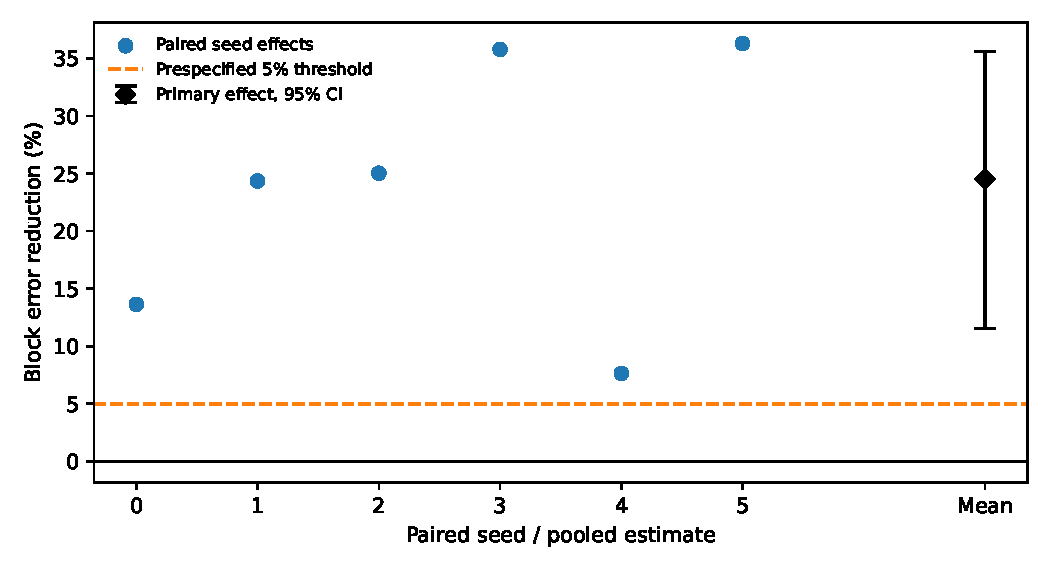
\includegraphics[width=.95\linewidth]{../reports/figures/paired_effects.pdf}\caption{All six paired seed effects and the primary transformed t confidence interval. The dashed line is the prespecified practical threshold.}\end{figure}
\begin{table}[ht]\centering\small
\begin{tabular}{lll}
\toprule
Model & Convection & Radiative \\
\midrule
GPhyT without Attention Residuals & 39284.2 & 0.392769 \\
GPhyT + Block AttnRes & 30006 & 0.289174 \\
\bottomrule
\end{tabular}
\caption{Primary baseline comparison: arithmetic mean twelve-step NMSE across the same six seeds (lower is better). Both models train from scratch with identical shared-parameter initialization, paired sampled examples, optimizer schedule, update count, and effective batch size. Compute cost differs by architecture. The preregistered two-dataset relative reduction uses paired dataset log-error ratios, not the ratio of these arithmetic means.}\end{table}
\begin{table}[ht]\centering\small
\begin{tabular}{llllll}
\toprule
Dataset & Model & Finite/planned & 1 step & 12 step & 24 step \\
\midrule
Convection & No AttnRes & 6/6 & 334.8 & 3.928e+04 & 4.561e+04 \\
Convection & Block & 6/6 & 181.8 & 3.001e+04 & 4.076e+04 \\
Convection & Full & 3/3 & 93.01 & 1.84e+04 & 3.126e+04 \\
Convection & Uniform & 3/3 & 200.6 & 2.499e+04 & 2.898e+04 \\
Convection & Persistence & 1/1 & 0.04142 & 0.2174 & 0.3296 \\
Radiative & No AttnRes & 6/6 & 0.1422 & 0.3928 & 0.7028 \\
Radiative & Block & 6/6 & 0.1332 & 0.2892 & 0.427 \\
Radiative & Full & 3/3 & 0.1381 & 0.3174 & 0.4357 \\
Radiative & Uniform & 3/3 & 0.1446 & 0.3473 & 0.5948 \\
Radiative & Persistence & 1/1 & 0.1529 & 0.419 & 0.5403 \\
\bottomrule
\end{tabular}
\caption{Arithmetic mean seed NMSE for each fixed horizon. No AttnRes denotes GPhyT without Attention Residuals. A horizon averages all forecast steps up to that horizon. Architecture means require every planned seed to have a finite endpoint. Finite/planned counts refer to twelve steps; persistence is a deterministic baseline, not a one-seed uncertainty estimate. Complete descriptive seed SDs and t intervals are in accuracy\_summary.csv.}\end{table}
\begin{figure}[ht]\centering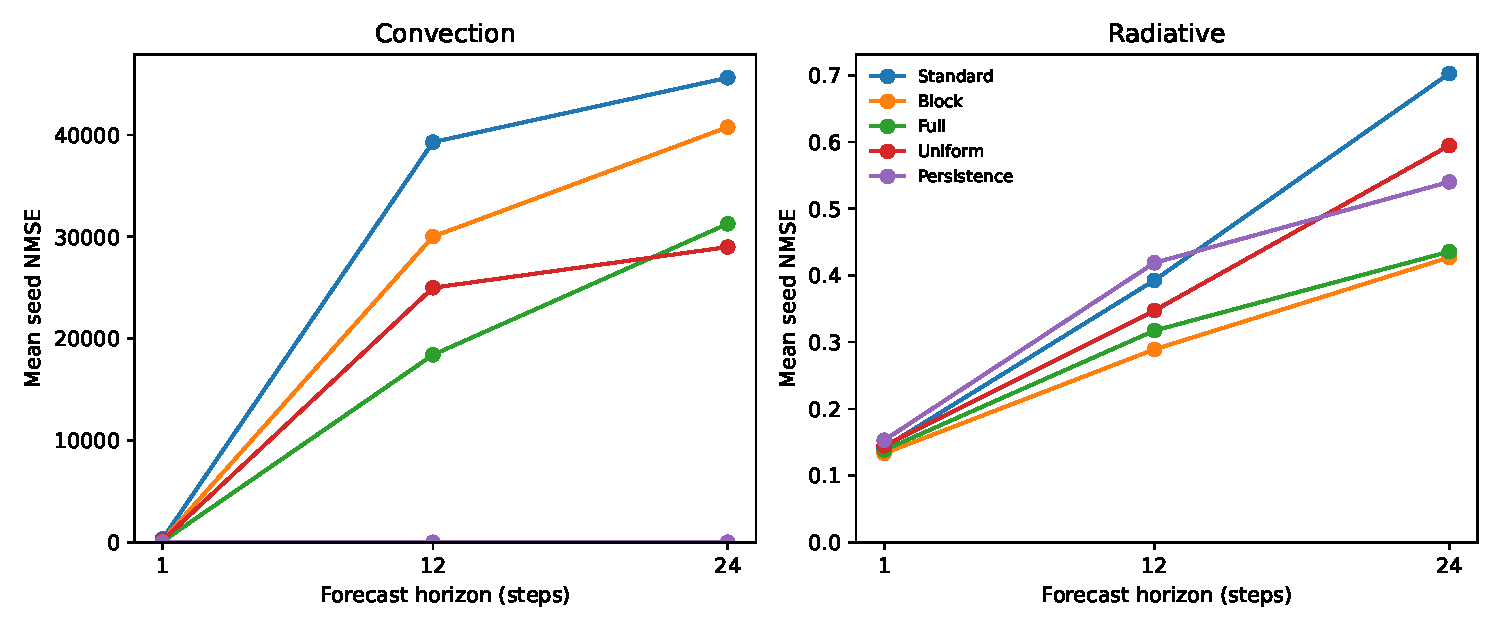
\includegraphics[width=\linewidth]{../reports/figures/forecast_errors.pdf}\caption{Fixed-horizon trajectory-averaged errors for both datasets. Missing values remain missing.}\end{figure}
\begin{table}[ht]\centering\scriptsize
\begin{tabular}{lrrrr}
\toprule
Run & Updates & Wall seconds & Examples/s & Peak MiB \\
\midrule
block\_seed0 & 3175 & 2473.97 & 20.68 & 365.88 \\
block\_seed1 & 3175 & 2011.53 & 25.65 & 365.88 \\
block\_seed2 & 3175 & 2639.13 & 19.30 & 365.88 \\
block\_seed3 & 3175 & 2547.29 & 20.36 & 365.88 \\
block\_seed4 & 3175 & 2522.62 & 20.63 & 365.88 \\
block\_seed5 & 3175 & 2568.18 & 20.49 & 365.88 \\
full\_seed0 & 3175 & 2966.65 & 18.11 & 546.00 \\
full\_seed1 & 3175 & 2829.46 & 18.36 & 546.00 \\
full\_seed2 & 3175 & 2473.04 & 20.80 & 546.00 \\
standard\_seed0 & 3175 & 2191.09 & 26.75 & 278.46 \\
standard\_seed1 & 3175 & 1282.01 & 41.12 & 278.46 \\
standard\_seed2 & 3175 & 1510.54 & 33.42 & 278.46 \\
standard\_seed3 & 3175 & 1459.29 & 35.46 & 278.46 \\
standard\_seed4 & 3175 & 1488.47 & 35.03 & 278.46 \\
standard\_seed5 & 3175 & 1490.51 & 34.76 & 278.46 \\
uniform\_block\_seed0 & 3175 & 2655.30 & 20.01 & 345.86 \\
uniform\_block\_seed1 & 3175 & 2470.89 & 21.12 & 345.86 \\
uniform\_block\_seed2 & 3175 & 2238.16 & 23.09 & 345.86 \\
\bottomrule
\end{tabular}
\caption{Per-run cost, including failed or incomplete runs. Examples/s uses the median synchronized update time; wall seconds also include validation and checkpointing. Peak memory is PyTorch allocated device memory.}\end{table}
\begin{table}[ht]\centering\small
\begin{tabular}{lll}
\toprule
Model / routing control & Convection & Radiative \\
\midrule
Block: original & 17550.8 & 0.297138 \\
Block: uniform intervention & 42767.8 & 2.16975 \\
Block: shuffled (random) intervention & 40924 & 2.81369 \\
\bottomrule
\end{tabular}
\caption{Absolute twelve-step NMSE on the matched diagnostic subset: first four test trajectories per dataset, averaged across all six trained Block seeds. The original reference is evaluated on exactly this subset, not the full test population in the baseline tables. Uniform replaces routing weights by equal weights; shuffled is the random control, permuting learned depth-weight assignments with RNG seed 20261025. Neither intervention is retrained. Seed counts, SDs, and descriptive intervals are in intervention\_accuracy\_summary.csv.}\end{table}
\begin{table}[ht]\centering\small
\begin{tabular}{lllrr}
\toprule
Dataset & Routing & Finite/planned & Mean error ratio & Seed SD \\
\midrule
Convection & shuffle & 6/6 & 2.63 & 1.245 \\
Convection & uniform & 6/6 & 2.565 & 0.7757 \\
Radiative & shuffle & 6/6 & 9.524 & 5.603 \\
Radiative & uniform & 6/6 & 7.49 & 6.105 \\
\bottomrule
\end{tabular}
\caption{Within-model twelve-step routing interventions on the same first four test trajectories per dataset. Values are intervened/original NMSE ratios, averaged over trained Block seeds. These are exploratory diagnostics, not independently trained controls or evidence of a unique mechanism.}\end{table}
\begin{table}[ht]\centering\scriptsize
\begin{tabular}{llrrr}
\toprule
Dataset & Diagnostic & Standard & Block & Persistence \\
\midrule
Convection & Divergence error RMS & 4.13 & 2.82 & 0.228 \\
Convection & Predicted divergence RMS & 4.13 & 2.81 & 0.165 \\
Convection & Target divergence RMS & 0.175 & 0.175 & 0.175 \\
Radiative & Negative density fraction & 0.26 & 0.273 & 0 \\
Radiative & Negative pressure fraction & 0 & 0 & 0 \\
\bottomrule
\end{tabular}
\caption{Secondary physical diagnostics averaged over all 24 forecast steps, then windows, trajectories, and complete planned seed sets. Divergence uses the stored physical coordinates and coarsened target; positivity rates are fractions. These diagnostics do not establish exact conservation. All architectures and interventions are retained in physical\_diagnostics.csv.}\end{table}
Across the available ordinary evaluations, 0/1368 forecast windows have undefined twelve-step error, and 0/1368 have undefined twenty-four-step error. These descriptive counts include persistence and repeated model evaluations; they are not independent replicates or an inferential sample size. Per-run counts are preserved in rollout\_stability.csv.
\begin{figure}[ht]\centering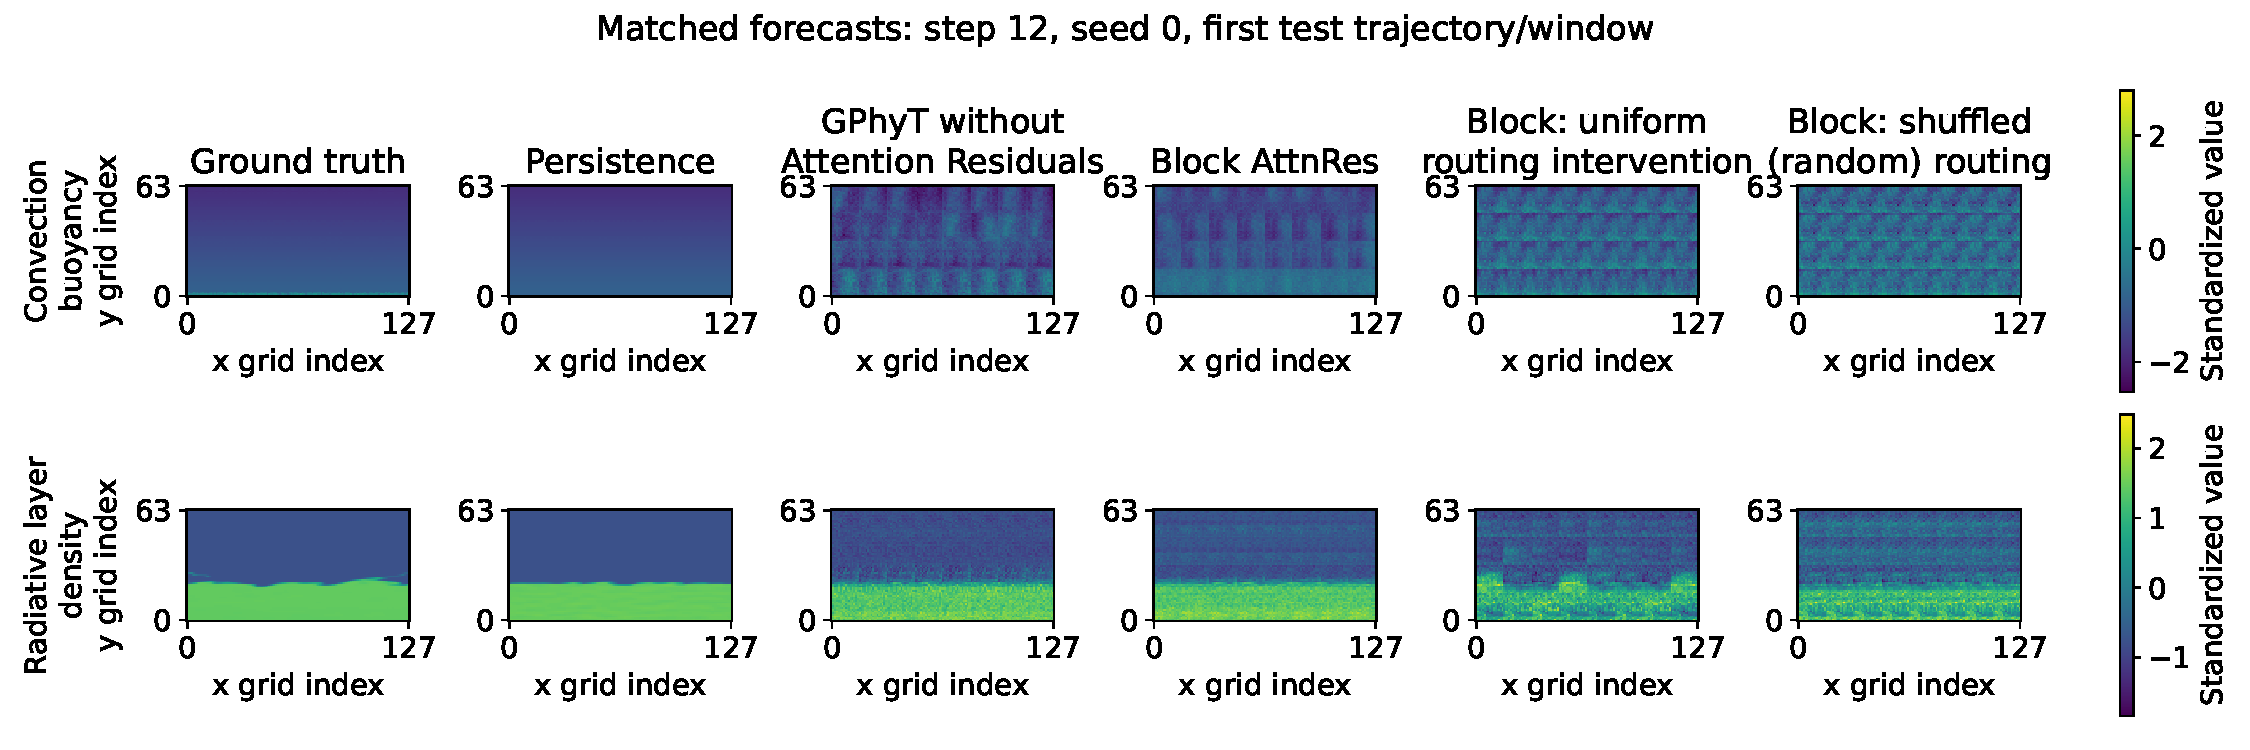
\includegraphics[width=\linewidth]{../reports/figures/control_comparison.pdf}\caption{Baselines, new method, and controls on the same first test trajectory/window at step twelve: persistence, GPhyT without Attention Residuals, ordinary Block, and Block with uniform or randomly shuffled depth weights. Interventions use the same trained seed-zero Block checkpoint without retraining; shuffling preserves learned weight magnitudes but permutes source assignments with fixed RNG seed 20261025. Persistence repeats the last observed context frame. Rows show convection buoyancy and radiative density with one shared, unclipped color scale per row in training-standardized units. This post-result presentation reuses fixed cases and saved intervention forecasts; it introduces no new endpoint or GPU inference.}\end{figure}
\begin{figure}[ht]\centering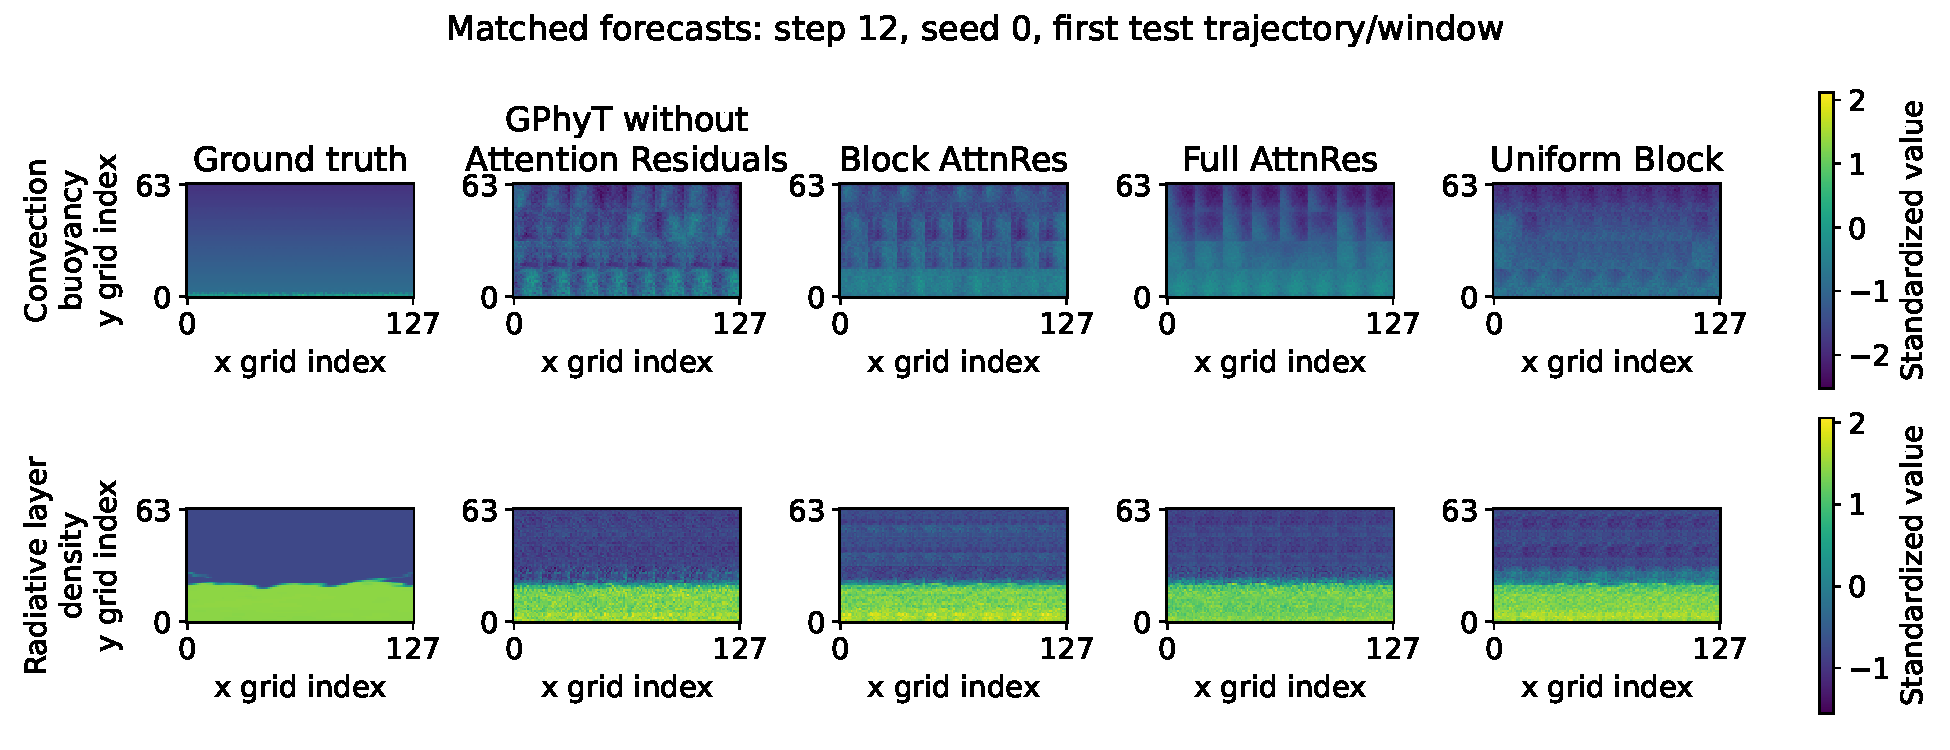
\includegraphics[width=\linewidth]{../reports/figures/field_comparison.pdf}\caption{Ground truth and all four trained architectures on identical held-out cases: seed zero, first test trajectory and first fixed window, forecast step twelve. Each row uses one common color range spanning truth and all predictions, without clipping, in training-standardized units; magenta would mark nonfinite values. Convection shows buoyancy (not temperature); radiative flow shows density. These illustrative fields do not replace the full paired evaluation. The all-model layout was added after results at the user's request, reusing the already fixed preview cases.}\end{figure}
\begin{figure}[ht]\centering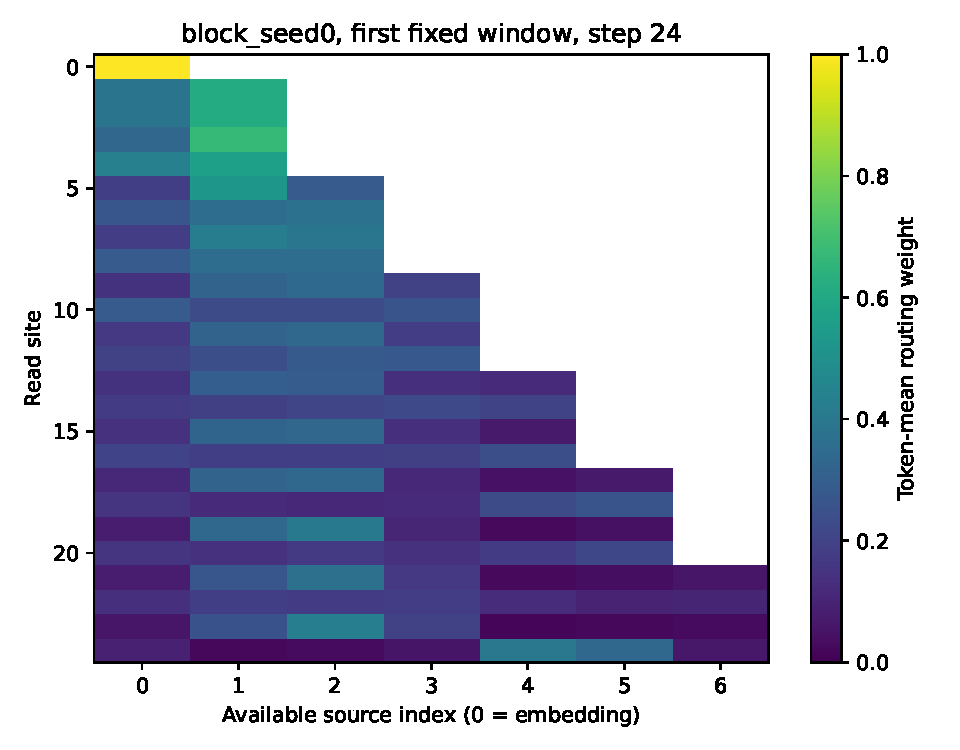
\includegraphics[width=.72\linewidth]{../reports/figures/routing_block_seed0.pdf}\caption{Routing in the prespecified seed-zero, first-trajectory, first-window case. White cells represent unavailable or undefined weights; a heatmap alone does not establish causal importance.}\end{figure}
\begin{figure}[ht]\centering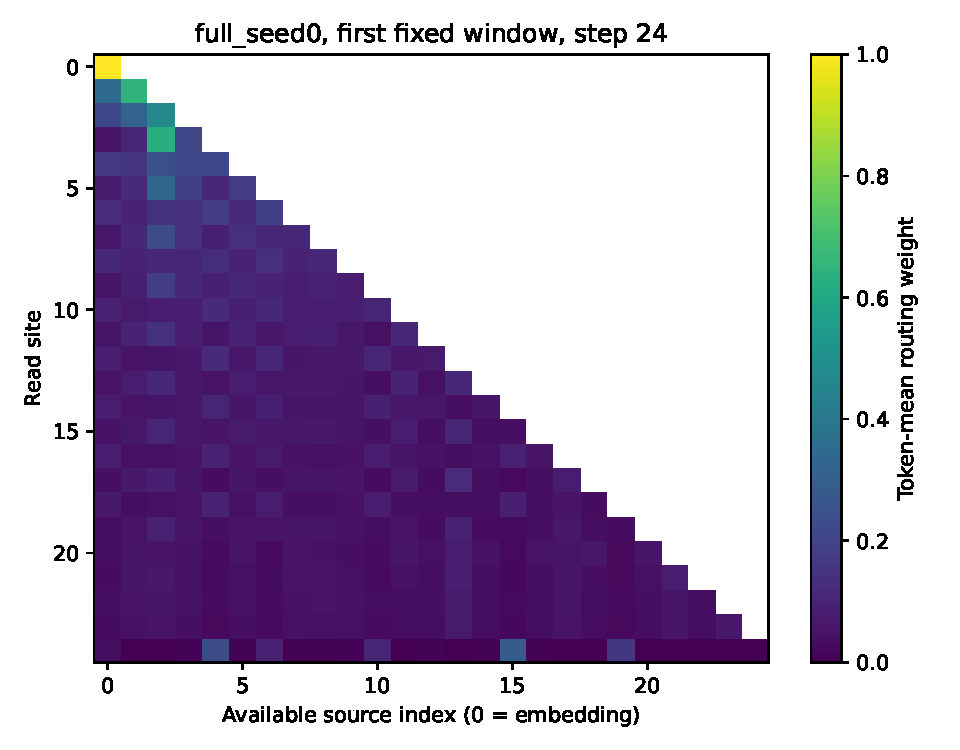
\includegraphics[width=.72\linewidth]{../reports/figures/routing_full_seed0.pdf}\caption{Routing in the prespecified seed-zero, first-trajectory, first-window case. White cells represent unavailable or undefined weights; a heatmap alone does not establish causal importance.}\end{figure}
\begin{figure}[ht]\centering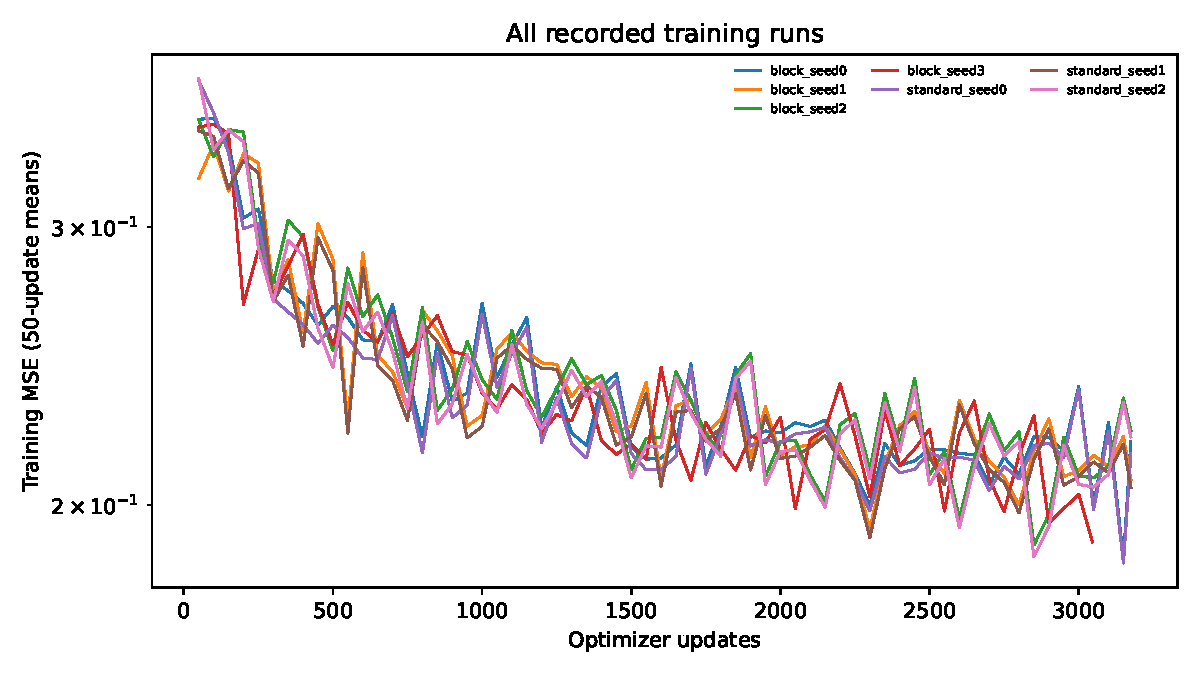
\includegraphics[width=\linewidth]{../reports/figures/learning_curves.pdf}\caption{All recorded runs with fixed fifty-update bins. Full update records accompany the checkpoints. Supervised MSE is a training objective, not a reinforcement-learning reward.}\end{figure}
\begin{figure}[ht]
\centering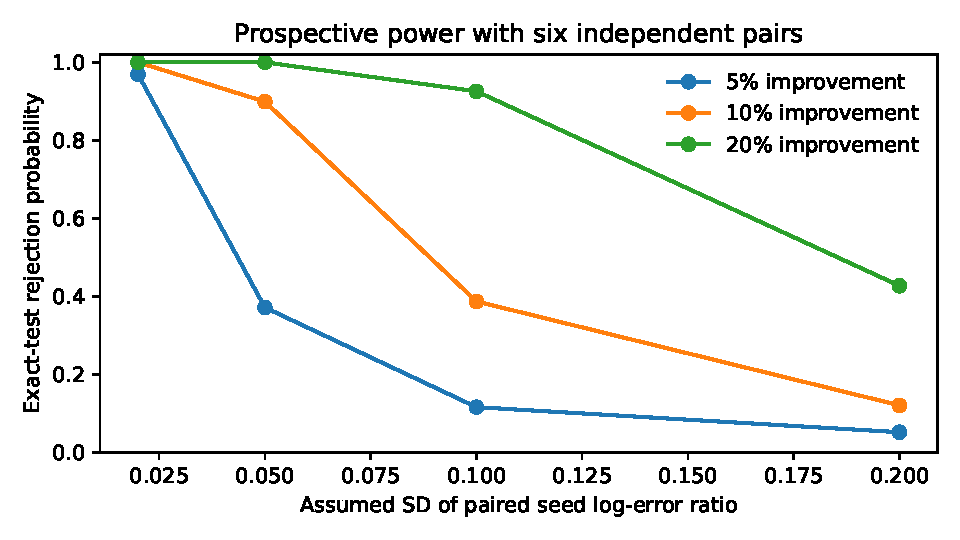
\includegraphics[width=.8\linewidth]{../reports/figures/power_sensitivity.pdf}
\caption{Prospective power under explicitly assumed independent Gaussian seed effects. This is a sensitivity calculation, not observed prediction accuracy.}\end{figure}
For a 5\% improvement, exact-test simulated power is 0.37124 at assumed log-ratio standard deviation 0.05 and 0.11563 at 0.10 (100,000 draws per condition). All sensitivity assumptions and Monte Carlo errors are published.
\clearpage
\subsection{Post-hoc initialization-only baselines}
The additional user-requested zero-update evaluation completed 18/18 planned controls. These controls were specified after observing the trained-model results and do not alter the original confirmatory comparison. The models were reconstructed with the original constructor, configuration, and seeds, without loading trained weights or applying optimizer updates. Parameter and buffer hashes were checked before and after inference.
\begin{table}[ht]\centering\scriptsize
\begin{tabular}{lllll}
\toprule
Dataset & Model & Finite/planned & Initialized & Trained \\
\midrule
Convection & GPhyT without AttnRes & 6/6 & 350742 & 39284.2 \\
Convection & Block AttnRes & 6/6 & 8173.5 & 30006 \\
Convection & Full AttnRes & 3/3 & 1332 & 18397.8 \\
Convection & Uniform Block & 3/3 & 7780.76 & 24987 \\
Radiative & GPhyT without AttnRes & 6/6 & 7.02088 & 0.392769 \\
Radiative & Block AttnRes & 6/6 & 0.572704 & 0.289174 \\
Radiative & Full AttnRes & 3/3 & 0.413095 & 0.317353 \\
Radiative & Uniform Block & 3/3 & 0.524838 & 0.347345 \\
\bottomrule
\end{tabular}
\caption{Twelve-step NMSE for initialized models (zero updates) and their trained counterparts (3,175 updates), on the same complete test population. Standard/Block use seeds 0--5; Full/Uniform use seeds 0--2. Finite/planned counts refer to initialized endpoints; incomplete or divergent seed sets remain undefined. These are descriptive post-hoc controls, not additional confirmatory tests. All horizons and seed uncertainty are in reports/untrained/comparison.csv.}\end{table}
\begin{figure}[ht]\centering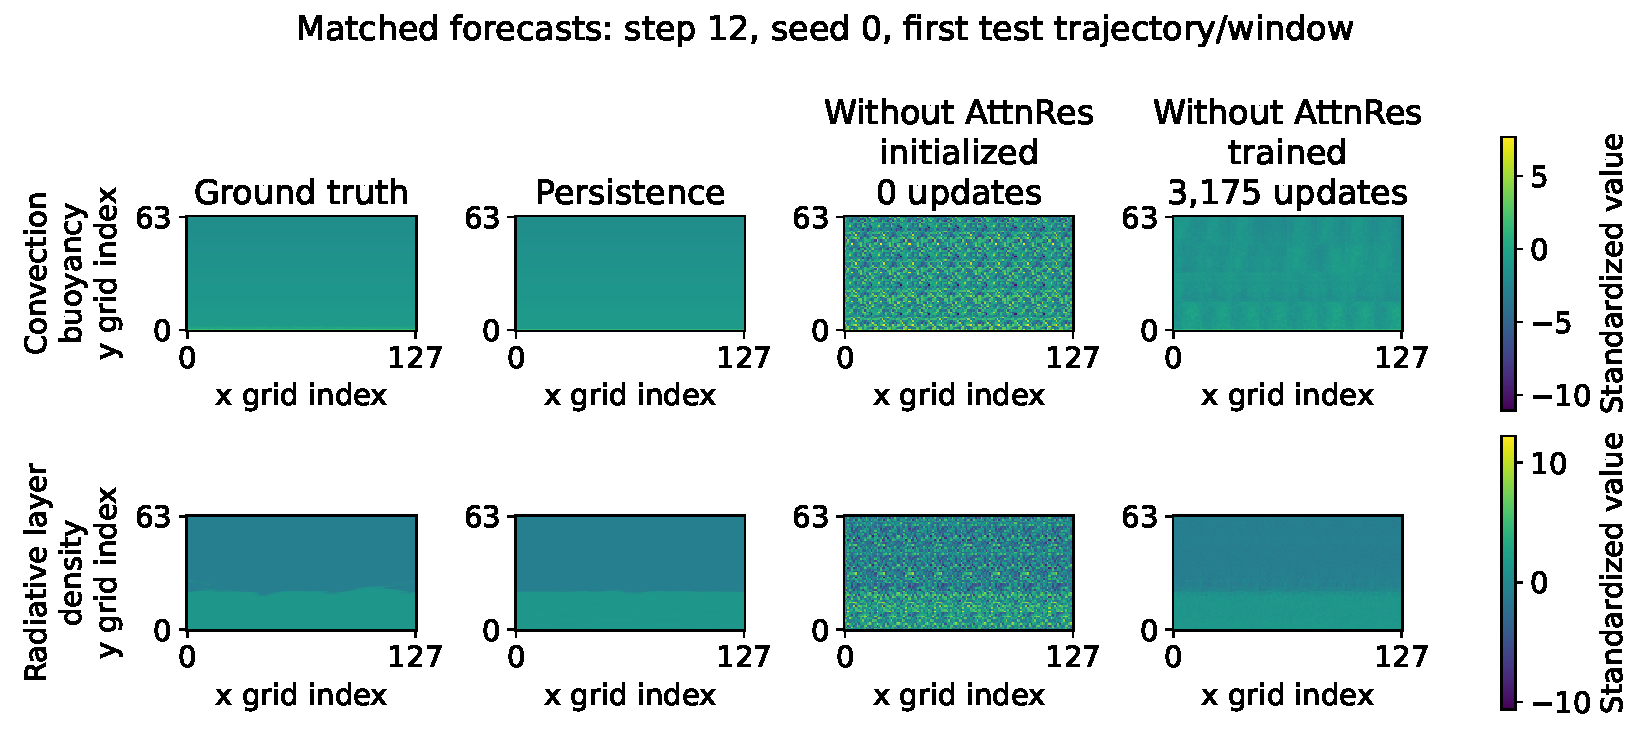
\includegraphics[width=\linewidth]{../reports/figures/initialization_standard.pdf}\caption{Initialized versus trained GPhyT without AttnRes: ground truth, persistence, zero-update model, and final trained checkpoint. Both rows use the same seed-zero first test trajectory/window at forecast step twelve, with one common unclipped color range per row. Top: convection buoyancy; bottom: radiative density. Magenta denotes nonfinite values. These fixed illustrative cases do not replace evaluation over all trajectories and seeds.}\end{figure}
\begin{figure}[ht]\centering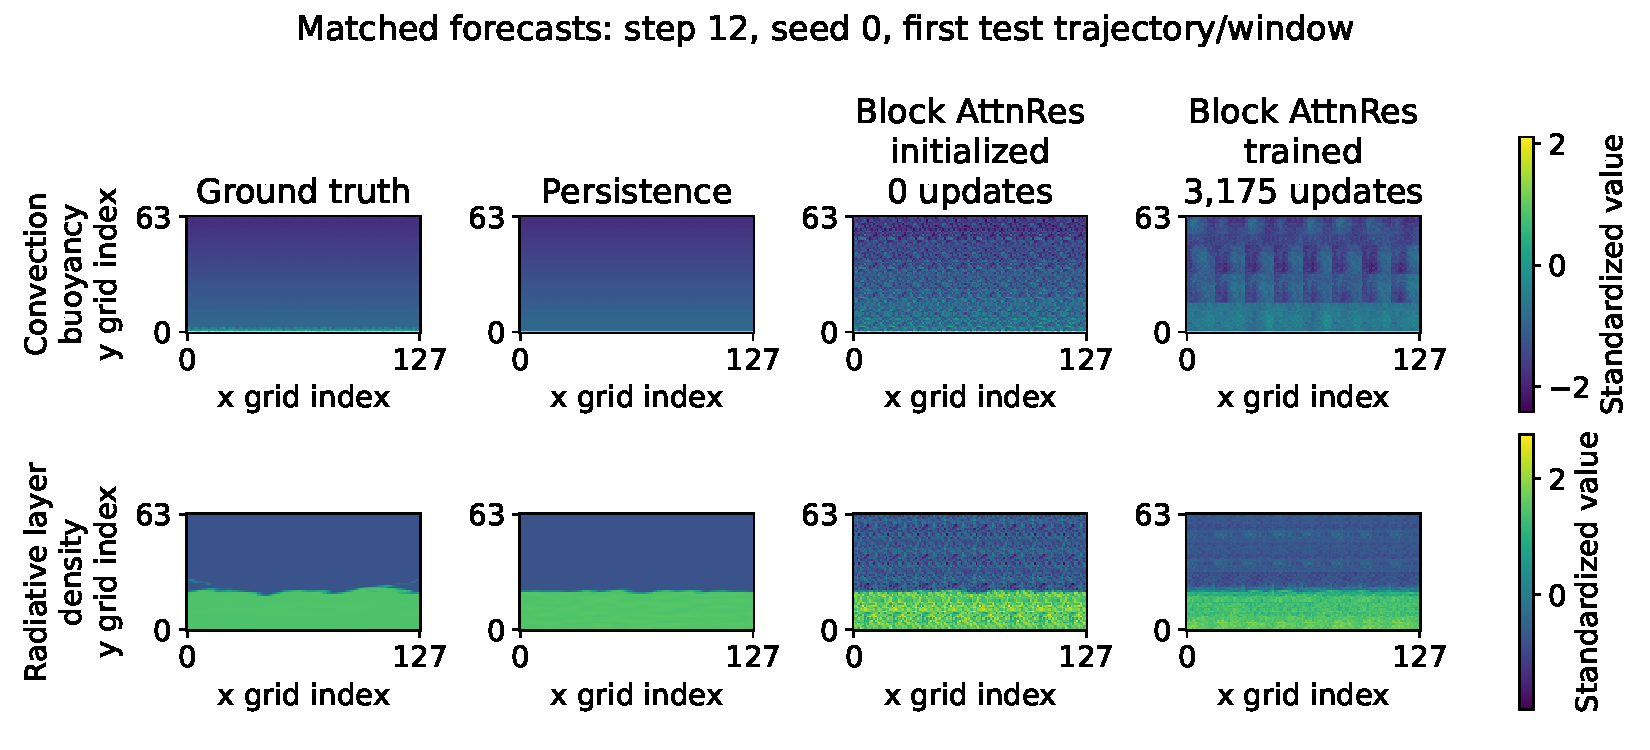
\includegraphics[width=\linewidth]{../reports/figures/initialization_block.pdf}\caption{Initialized versus trained Block AttnRes: ground truth, persistence, zero-update model, and final trained checkpoint. Both rows use the same seed-zero first test trajectory/window at forecast step twelve, with one common unclipped color range per row. Top: convection buoyancy; bottom: radiative density. Magenta denotes nonfinite values. These fixed illustrative cases do not replace evaluation over all trajectories and seeds.}\end{figure}
\begin{figure}[ht]\centering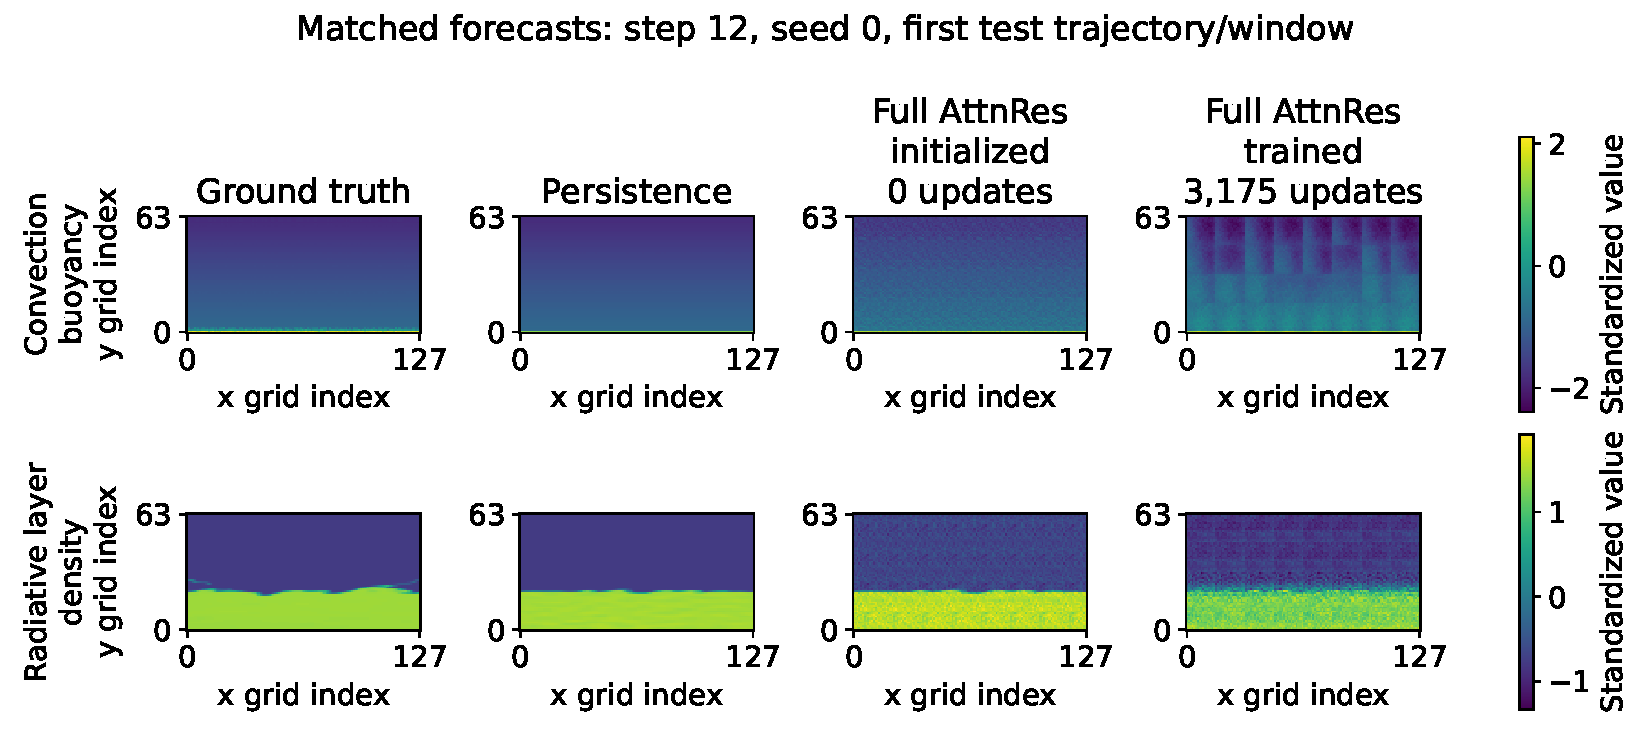
\includegraphics[width=\linewidth]{../reports/figures/initialization_full.pdf}\caption{Initialized versus trained Full AttnRes: ground truth, persistence, zero-update model, and final trained checkpoint. Both rows use the same seed-zero first test trajectory/window at forecast step twelve, with one common unclipped color range per row. Top: convection buoyancy; bottom: radiative density. Magenta denotes nonfinite values. These fixed illustrative cases do not replace evaluation over all trajectories and seeds.}\end{figure}
\begin{figure}[ht]\centering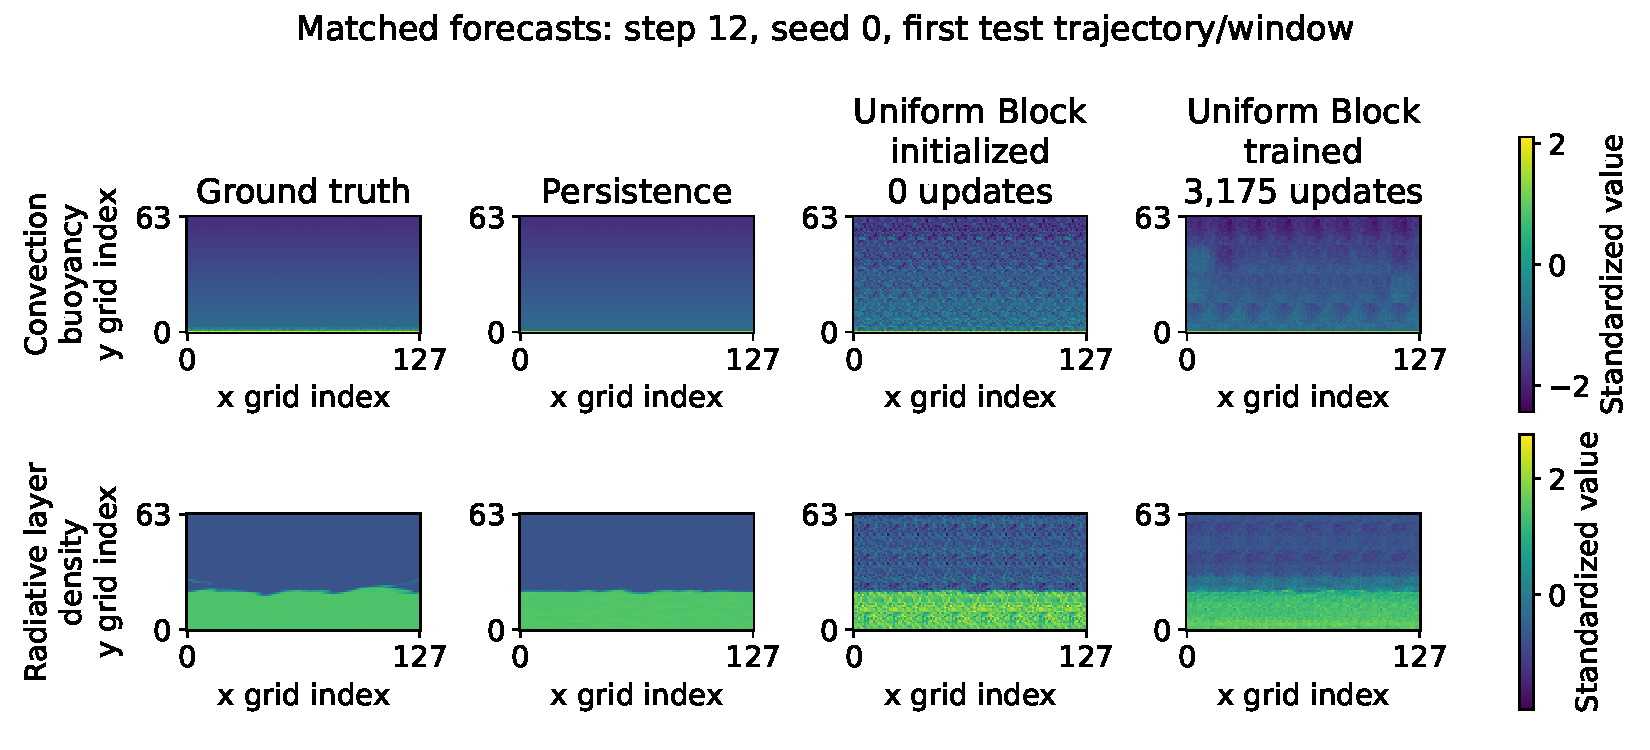
\includegraphics[width=\linewidth]{../reports/figures/initialization_uniform_block.pdf}\caption{Initialized versus trained Uniform Block: ground truth, persistence, zero-update model, and final trained checkpoint. Both rows use the same seed-zero first test trajectory/window at forecast step twelve, with one common unclipped color range per row. Top: convection buoyancy; bottom: radiative density. Magenta denotes nonfinite values. These fixed illustrative cases do not replace evaluation over all trajectories and seeds.}\end{figure}
